\documentclass[12pt,a4paper]{article}
\synctex=1
\usepackage[utf8]{inputenc}
\usepackage[margin=1cm]{geometry}
\usepackage{graphicx}
%\usepackage{verbatim}
\usepackage{listings}
\usepackage{textcomp}
\usepackage{courier}
\usepackage{libertine}
\usepackage{pgfornament}
\usepackage{eso-pic}
\usepackage[hangul]{kotex}
\linespread{1.3}

\title{
	\centering
	\pgfornament[width=12cm,color=teal]{84}\\
	\vspace{1cm}
	\fontsize{50}{50} \selectfont {컴퓨터 알고리즘과 실습}\\
		\pgfornament[width=12cm,color=teal]{88}\\
	\vfill}
\author{
	\LARGE
	\begin{tabular}{rl}
		\hline
		학번 : & 2016110056\\ 
		학과 : & 불교학부 \\
		이름 : & 박승원\\
		날짜 : & \today\\
		\hline
	\end{tabular}\vspace{2cm}
	\\
\includegraphics[width=0.5\textwidth]{logo.jpg}
	}
\date{}


\begin{document}
\maketitle
\pagenumbering{gobble}
\noindent
\lstset{language=C++, columns=flexible, tabsize=4, frame=shadowbox, showstringspaces=false, breaklines=true, upquote=true, basicstyle=\normalsize}

\includegraphics[page=3, width=\textwidth]{1.pdf}
\lstinputlisting{1.cpp}

\includegraphics[width=\textwidth]{1.png}

\includegraphics[page=6, width=\textwidth]{1.pdf}
\lstinputlisting{2.cpp}

\includegraphics[width=\textwidth]{2.png}

\includegraphics[page=7, width=\textwidth]{1.pdf}
\includegraphics[page=8, width=\textwidth]{11.pdf}
\includegraphics[page=9, width=\textwidth]{11.pdf}
대각선으로 각 지점에 도달하는데에 걸리는 에지의 웨이트를 합하여 최고값을 쓴다.
대각선을 도착지점을 향하여 전진시키며 위를 반복한다.
다익스트라 알고리즘의 경우 음수로 웨이트를 변형하여 계산을 해보았으나, 다익스트라 알고리즘은 음수가 아닌 경우에만 최소 경로를 찾을 수가 있었다.
롱기스트 패스를 찾는 일반적인 문제는 NP완전문제로 아직까지 그 해법이 알려지지 않았다.\\

for i 1 to 5 : for j 1 to 5 :\\
$S_{i,j} \leftarrow max(\overrightarrow{W}_{i}+S_{i-1,j}, 
S_{i,j-1}+W_j$\textdownarrow)


\end{document}
